% Template by David Madras, inspired by Meltem Atay's template for the 2018 SOCML

\documentclass{article}
\usepackage{enumitem}
\usepackage{dsfont}
\usepackage{amsmath}
\usepackage{tikz}
\usetikzlibrary{shapes.geometric, positioning}
\usepackage{rotating}
\usepackage{amsfonts}
\title{Variational Autoencoders Derivation}
\author{Jacob Yeung}
\date{August 28, 2020}

\begin{document}

\maketitle

Note detailing derivation of variational autoencoders (VAEs). Also first attempt at writing notes in LaTeX.

\section{Brief Background}
Autoencoders are a technique for dimensionality reduction, akin to PCA, but allow for more complex features because of non-linearities that can be utilized. We can use a neural network to reduce dimensionality to prevent memorization of input (identity mapping). There are several types of autoencoders - basic, sparse, denoising. This note focuses on VAEs.

\section{Derivation}
\subsection{Basic Probability}
\begin{itemize}
    \item Information := $-\text{log}(P(x))$
    \begin{itemize}
        \item This makes intuitive sense - consider $x$ describes probability of my dog crying and not crying. Probability of $x$ occurring is 1, which gives me no useful information.
        \item Low prob. $x$ gives lots info
    \end{itemize}
    \item Entropy := $-\sum P(x)\text{log}P(x)$
    \item Kullback–Leibler (KL) divergence KL$(p\parallel q)$ = $-\sum p(x)\text{log}\frac{p(x)}{q(x)}$
    \begin{itemize}
        \item KL divergence tells us how similar two probability distributions are w.r.t. first distr. - similar to measuring difference between two distr.
        \item Intuitive first step: $-\sum q(x)\text{log}q(x) + \sum p(x)\text{log}p(x)$ (incorrect)
        \item Tweak $-\sum p(x)\text{log}q(x) + \sum p(x)\text{log}p(x)$ (correct since distr. q w.r.t. p)
        \item Properties
        \begin{itemize}
            \item KL $\geq 0$
            \item KL$(p\parallel q) \ne \text{KL}(q\parallel p)$
        \end{itemize}
    \end{itemize}
\end{itemize}
\subsection{Variational Inference}
Suppose we have observation $x$ from hidden variable $z$. We want to know more about $z$ so we want \begin{equation*}\label{goal}
\begin{aligned}
    P(z|x) &= \frac{P(x|z)P(z)}{P(x)}\\
    &= \frac{P(x, z)}{P(x)}
\end{aligned}
\end{equation*}
However, in most cases $P(x)$ is intractable, so we want to approximate $P(z|x)$ with $q(z)$, a known tractable distribution.
\subsection{Minimize KL divergence}
We want to minimize KL divergence of below eq since this creates the best approximation.
\begin{equation*}\label{approx}
\begin{aligned}
    \text{KL}(q(z)\parallel p(z|x)) &= -\sum_z q(z)\text{log}\frac{p(z|x)}{q(z)}\\
    &= -\sum_z q(z) \text{log}\frac{\frac{p(x,z)}{p(x)}}{q(z)}\\
    &= - \sum_z q(z)\text{log}\frac{p(x,z)}{q(z)}\frac{1}{p(x)}\\
    &= - \sum_z q(z)\text{log}\frac{p(x,z)}{q(z)} + \sum_z q(z)\text{log}p(x)\\
    &= - \sum_z q(z)\text{log}\frac{p(x,z)}{q(z)} + \text{log}p(x)
\end{aligned}
\end{equation*}
Rearrange to find constant in terms of distr. dependents
\begin{equation*}\label{rearrange}
\begin{aligned}
    \text{log}p(x) &= \text{KL}(q(z)\parallel p(z|x)) + \sum_z q(z)\text{log}\frac{p(x,z)}{q(z)}\\
    &= \text{KL}(q(z)\parallel p(z|x)) +\mathcal{L}
\end{aligned}
\end{equation*}
We define our second term as the variational lower bound since $\mathcal{L}\leq \text{log}p(x)$.

\subsection{Maximizing Variational Lower Bound}
Since $p(x)$ is a constant, minimzing our KL divergence is equivalent to maximizing $\mathcal{L}$.
\begin{equation}\label{L}
\begin{aligned}
    \mathcal{L} &= \sum q(z) \text{log}\frac{p(x,z)}{q(z)}\\
    &= \sum q(z) \text{log}\frac{p(x|z)p(x)}{q(z)}\\
    &= \sum q(z)\text{log} p(x|z) + \sum q(z) \text{log}\frac{p(z)}{q(z)}\\
    &= \mathbb{E}_{q(z)}p(x|z) -KL(q(z)\parallel p(z))
\end{aligned}
\end{equation}
Thus, we want to maximize the expectation and minimize the KL divergence.

\section{Application to VAEs}
We can treat our decoder as $q(z|x)$ mapping $x$ to $z$, and our encoder as $p(x|z)$ mapping z to $\tilde{x}$ where z is a vector of the latent variables.\\
\begin{center}
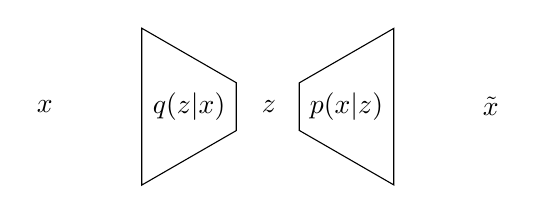
\begin{tikzpicture}
    \node[draw, trapezium, shape border rotate=270, minimum height=1.2cm] (dum) at (1, 1.5) {$q(z|x)$};
    \node[left=of dum] {$x$};
    \node[right=of dum] at (0.8, 1.5) {$z$};
    \node[draw, trapezium, shape border rotate=90, minimum height=1.2cm] (dummy) at (3, 1.5) {$p(x|z)$};
    \node[right=of dummy] {$\tilde{x}$};
\end{tikzpicture}
\end{center}
The encoder is deterministic, so $p(x|z) \approx p(x|\tilde{x})$.
\subsection{Gaussian Example}
Let us assume $p(x)$ is roughly Gaussian. Then
\begin{equation*}
    p(x|\tilde{x}) = e^{-|x-\tilde{x}|^2}
\end{equation*}
The reconstruction error is as follows.
\begin{equation*}
    \mathbb{E}_{q(z)} = -|x-\tilde{x}|^2
\end{equation*}
Now we substitute the reconstruction error back into our lower bound and multiply by $-1$ to minimize it.
\begin{equation*}
    \min \mathcal{L} = |x-\tilde{x}|^2 + KL(q(z)\parallel \mathcal{N}(\mu,\Sigma))
\end{equation*}
Now, instead of learning the hidden features directly, the decoder network learns the mean and variance of each hidden feature.
\section{Sources}
\begin{itemize}
    \item Ali Ghodsi lecture: https://www.youtube.com/watch?v=uaaqyVS9-rM&feature=youtu.be&t=19m42s
    \item Jeremy Jordan: https://www.jeremyjordan.me/variational-autoencoders/
    \item Deep Learning Book http://www.deeplearningbook.org/contents/autoencoders.html
\end{itemize}{}

\end{document}
